\chapter{Collecte, compréhension et préparation des données.}
\epigraph{“Data! Data! Data!” he cried impatiently. “I can’t make bricks without clay.”}{Sherlock Holmes}
\subparagraph{}
Ce chapitre présente le processus d'acquisition des données et leur préparation pour les besoins d'analyse et de modélisation. Nous décrivons en premier lieu le paysage des données au moment du début de notre stage pour ensuite présenter les opération de consolidation, d'audit et d'extension que nous lui faisons subir.
\cleardoublepage
\newcommand{\reels}{\mathbb{R}}
	\section{Compréhension et préparation des données locales\protect\footnote{Données disponibles au sein du portail Business Intelligence de l'OCP}}
	\subsection{Compréhension des données locales}
	Comme rappelé dans la section \ref{CGP}. Les travaux de nos prédécesseurs dans leurs efforts de moderniser le portail \textit{Business Intelligence} de l'OCP se sont arrêtés à automatiser l'archivage des données se rapportant aux historiques de ventes en terme de prix et volumes en un premier lieu\cite{CHEMLAL} avant de concevoir le socle OLAP\footnote{le traitement analytique en ligne (OnLine Analytical Processing, OLAP)\nomenclature{\textbf{OLAP : }}{OnLine Analytical Processing} est un type d'application informatique orienté vers l'analyse sur-le-champ d'informations selon plusieurs axes, dans le but d'obtenir des rapports de synthèse} dans la vue de générer des rapports synthétiques concernant les historiques des échanges du marché des phosphates ensuite\cite{NACER}.\\
	Seules sont ainsi présentes les données concernant les échanges internationaux en terme de produits phosphatés et ceux-ci sont présents sous deux différentes formes de données.
					\begin{wrapfigure}[9]{r}{5 cm}
						\raggedleft
						\fbox{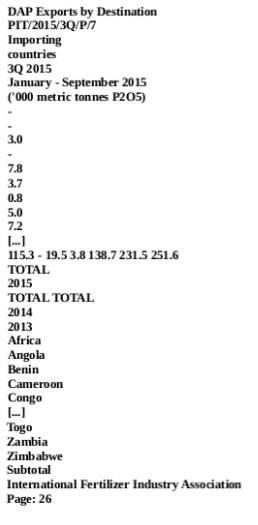
\includegraphics[scale=0.5]{ch3-images/IFA-txt}}
						\raggedleft
						\caption{Lecture "machine" du .pdf de la "Trade Matrix" de la figure \ref{fig:IFA-PDF}}
						\label{fig:IFA-TXT}
					\end{wrapfigure}
	La première est notre format de fichier source: des fichiers .pdf  non structurés vis-à-vis de notre besoin (figure \ref{fig:IFA-PDF}), et qui présentent:
		\begin{itemize}
		\item L'avantage d’être à jour, exhaustifs et dont la véracité est certifiée par un organisme international (IFA\nomenclature{\textbf{IFA : }}{International Fertilizer industry Association})
		\item L’inconvénient d’être flexible pour la lecture humaine mais ne présentant pas une grammaire machine formelle rendant possible une analyse syntaxique, comme en témoigne la figure \ref{fig:IFA-TXT}.
			\begin{figure}[H]
			    		\raggedright
		    			\fbox{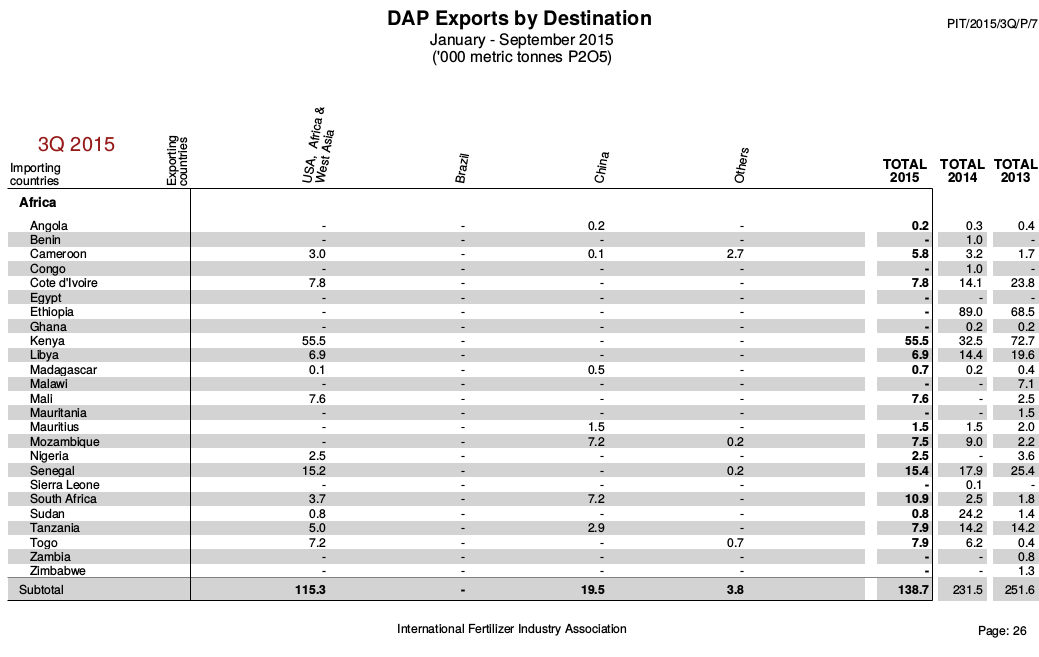
\includegraphics[scale=0.3]{ch3-images/IFA_EX}}
		    			\captionsetup{justification=raggedright,
		    			singlelinecheck=false
		    			}
			    		\caption{Exemple d'une "Trade Matrix"\protect\footnote{Matrice des imports/exports entre les pays du monde, deux-à-deux, des phosphates et produits dérivés} dans le rapport\\trimestriel de l'IFA}
			    		\label{fig:IFA-PDF}
			\end{figure}	
		\end{itemize}
		
		\paragraph{}
		La seconde est structurée dans des datamarts dont une sortie de requête est présentée dans la figure \ref{fig:DMOCP}.
	Ceci est notre format de données cible 
	et présente:
	\begin{itemize}
	\item L'avantage d’offrir le maximum de flexibilité pour le requêtage, et d'être de grande qualité en terme de disponibilité et de véracité, puisque celui-ci a été soigneusement introduit à la main\footnote{À travers une lecture "humaine" des .pdf présentés par la figure \ref{fig:IFA-PDF}}.
	\item L’inconvénient d'être prohibitif en temps et en ressources humaines.
	 En effet, nous avons constaté un retard datant de fin décembre 2013 par rapport aux derniers .pdf reçus par l'OCP.
	\end{itemize}
	\begin{figure}[H]
		    		\centering
	    			\fbox{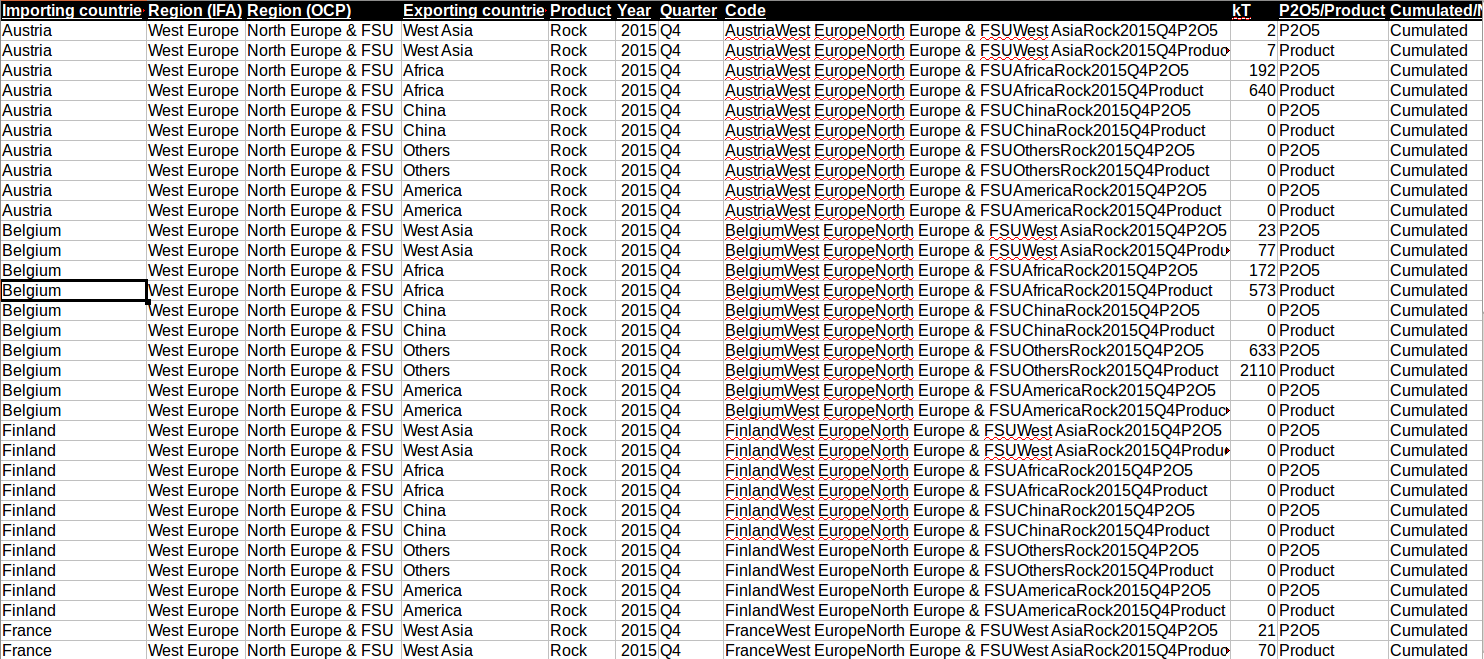
\includegraphics[scale=0.325]{ch3-images/Table}}
		    		\caption{Exemple d'une sortie de requête sur le Datamart OCP-CM}
		    		\label{fig:DMOCP}
	\end{figure}
	\subsection{Consolidation des données locales}
	Il est naturel d'adresser les problèmes de disponibilité de données aux premiers abords. La consolidation désigne la collection et l'intégration des données de sources multiples en une unique destination. Durant ce processus, nous unifierons les deux types de formats de données. Ceci nous permettra de présenter les données de manière plus flexible, tout en facilitant leur analyse effective. Ceci nous amène à considérer le format adopté par le datamart OCP-CM comme format cible de consolidation et les fichiers .pdf comme format source.
	\paragraph{}
	La solution que nous mettons en œuvre est disponible dans le dossier \textit{Sanxoriarty IFA Parser} du dépôt \textbf{GitHub} de notre mémoire de projet de fin d'études\cite{this}.
	\subsubsection{Conception fonctionnelle du processus de consolidation}
	L'OCP reçoit régulièrement des rapports trimestriels présentant la situation du marché accompagnée des mouvements observés des produits fertilisants. Ces mouvements sont reportés sur des tableaux tel que celui présenté dans la figure \ref{fig:IFA-PDF}. Notre solution doit ainsi considérer les nuances fonctionnelles suivantes :\newpage
	\begin{enumerate}
	\item Les rapports diffèrent par leur granularité. En effet ceux-ci peuvent être:
		\begin{itemize}
		\item DET : Détaillés. Présentant l'historique des mouvements de produits entre les pays du monde deux-à deux.
		\begin{figure}[h]
					    		\centering
					    		\fbox{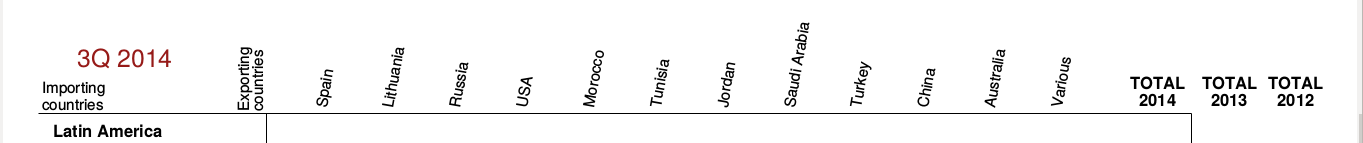
\includegraphics[scale=0.35]{ch3-images/det}}
					    		\caption{Exemple d'en-tête des tables du format DET des rapports IFA.}
				\end{figure}
		\item AGG : Agrégés. Présentant l'historique des mouvements entre les pays agrégés selon la région du monde à laquelle ceux-ci appartiennent.
		\begin{figure}[h]
			    		\centering
			    		\fbox{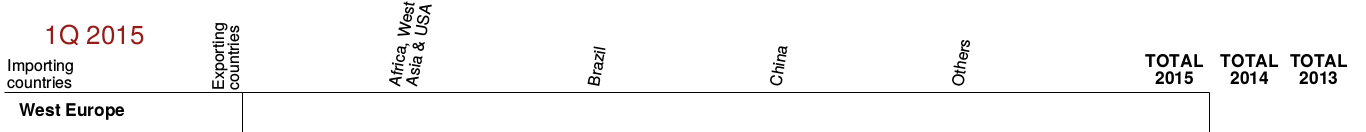
\includegraphics[scale=0.35]{ch3-images/agg}}
			    		\caption{Exemple d'en-tête des tables du format  AGG des rapports IFA.}
		\end{figure}
		\end{itemize}
	\item Les rapports diffèrent par les normes des chiffres rapportés. En effet ceux-ci peuvent être:
		\begin{itemize}
		\item NOT CUMULATED : Les chiffres rapportés au trimestre ${Q_i}$ sont bruts et représentent uniquement les ventes ayant effectivement eu lieu durant ce trimestre.
		\item CUMULATED : Les chiffres rapportés au trimestre ${Q_i}$ sont cumulés, i.e ${Q_i = \sum_{j=1}^{j=i} Q_j}$
		\item ANN : Les chiffres rapportés représentent toutes les ventes de l'année, i.e ${Q_i = \sum_{j=1}^{j=4} Q_j}$
		\end{itemize}
	\item Les attributs des enregistrements du datamart OCP-CM, sont des champs obligatoirement \textbf{NOT NULL} et sont les suivants:
	\begin{itemize}
	\item "Importing.countries" : Pays de destination de l'enregistrement-vente.
	\item "Region..IFA." : Région à laquelle appartient le pays de destination selon le découpage IFA.
	\item "Region..OCP." : Région à laquelle appartient le pays de destination selon le découpage OCP.
	\item "Exporting.countries" : Pays d'origine de l'enregistrement-vente.
	\item "Product" : Produit de l'enregistrement-vente. (MAP, DAP,PA\nomenclature{\textbf{PA : }}{Acide phosphorique},TSP ,Rock\footnote{Minerai du phosphate brut en roche.})
	\item "Year" : Année de l'enregistrement-vente.
	\item "Quarter" Trimestre de l'enregistrement-vente.
	\item "Code" : Code de Synthèse des champs précédents.
	\item "kT" :  Poids de l'enregistrement-vente en kT\footnote{Kilotonne = $10^6$ kilogramme.}.           
	\item "P2O5.Product" : Drapeau indiquant si le poids indiqué à la colonne \textit{kT}est net en P2O5\footnote{Pentoxyde de phosphore, la molécule de base des engrais phosphatés} ou en poids brut.
	\item "Cumulated.Not.cumulated" : Drapeau indiquant la norme trimestrielle de l'enregistrement-vente.
	\item "AGG.DET.ANN" : Drapeau indiquant la granularité de l'enregistrement-vente
	\end{itemize}
		Ainsi au-delà de la lecture des données contenues au sein des documents .pdf, ceux-ci doivent être:
		\begin{itemize}
		\item \textbf{Décumulés:} Des enregistrement des volumes unitaires par trimestre doivent être créés.
		\item \textbf{Convertis en P2O5:} Les données contenues dans les .pdf représentent les volumes échangés par kT qu'ils faut convertir selon la concentration du produit de l'enregistrement-vente en P2O5.
		\item \textbf{Normés:} La nature de l'agrégation trimestrielle de l'enregistrement-vente doit être spécifiée.
		\end{itemize}
	\end{enumerate}
	\subsubsection{Conception technique du processus de consolidation}\label{parser}
	\par
	La collecte et la préparation des données est un processus extrêmement lent et complexe,			\begin{wrapfigure}[14]{c}{8.4 cm}
						    		
						    		\fbox{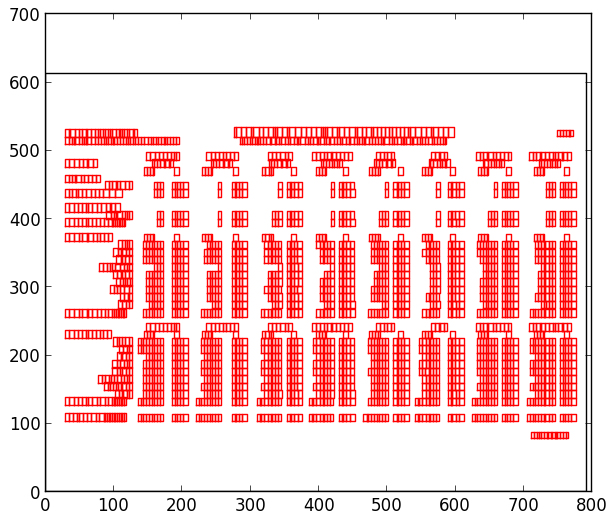
\includegraphics[scale=0.38]{ch3-images/charplot}}
						    		\caption{Représentation de l'information transportée par la page .pdf de la figure \ref{fig:IFA-PDF} pour une résolution d'image de 700x800.}
						    		\label{fig:charplot}
				\end{wrapfigure}  traditionnellement fait à la main et dont l'automatisation est souvent très difficile.
Le constat montre que 80 \% de la durée d'un projet Data Mining est consacrée à la récolte et la préparation des données\cite{DP}. Pour des données non structurées telles que des fichiers .pdf, la tâche est d'autant plus complexe. À la question : "Comment réaliser un \textit{Parsing} de fichiers PDFs", la réponse est souvent : "avec beaucoup de difficultés".

	\par
	PDF est un format de description de page et ne contient aucune information sur la structure logique d'un document telle que:\begin{itemize}
	\item L'emplacement du titre,
	\item Le début d'un paragraphe,
	\item Si la page est en une seule colonne ou plusieurs, etc.
	\end{itemize}
	\par
	Tout ce qu'un fichier .pdf indique est l'emplacement des caractères. La figure \ref{fig:charplot} ci-dessous montre comment les caractères sont disposés sur la page de la figure \ref{fig:IFA-PDF}.\\Une solution existe : \textbf{Tabula} de \textit{Mozilla} écrite en \textbf{Ruby} et précédemment utilisée par nos prédécesseurs (\cite{CHEMLAL},\cite{NACER}). Mais celle-ci présente l'inconvénient de nécessiter de l'utilisateur de dessiner des rectangles autour des tables cibles, ce qui n'offre aucun avantage d'automatisation.
	\par
	Notre solution utilise le package \textbf{pdfminer}\cite{pdfminer} du langage \textbf{Python} qui extrait les objets	\begin{wrapfigure}[16]{c}{8.4 cm}
			\centering			    		
			\fbox{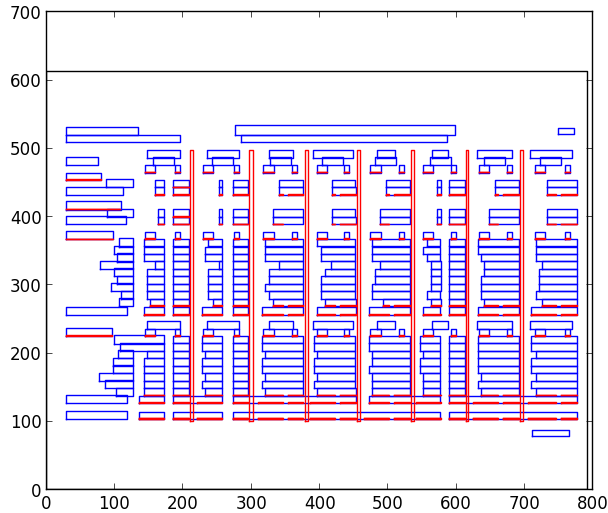
\includegraphics[scale=0.37]{ch3-images/classplot}}
			\caption{Classification de l'information transportée par la page .pdf de la figure \ref{fig:IFA-PDF}\\ selon ($\in$ zone de texte, $\notin$ zone de texte)}
			\label{fig:charclass}
		\end{wrapfigure}
		 non-texte et les mots de liaison en tant que blocs cohérents. Cette classification est montrée dans la figure \ref{fig:charclass} ci-contre. Les boîtes bleues indiquent où \textbf{pdfminer} a rassemblé un ensemble de caractères pour en faire des \textit{text boxes}\footnote{Zone de texte.} (cet ensemble de caractères peut être des mots ou des phrases) et les boites rouges indiquent les éléments non-texte (i.e, des lignes, des rectangles, etc.).
	\par
	La méthode utilisée par notre solution s'inspire des algorithmes d'analyse d'image et est similaire à la transformée de Hough utilisée par \textbf{Tabula}. Une transformée de Hough retrouve des segments de droites arbitrairement orientés dans une image. Notre problème, ici, est plus simple, nous nous intéressons uniquement au formes horizontales et verticales.
	\paragraph{}
	\begin{wrapfigure}[14]{c}{8.4 cm}
							\centering			    		
							\fbox{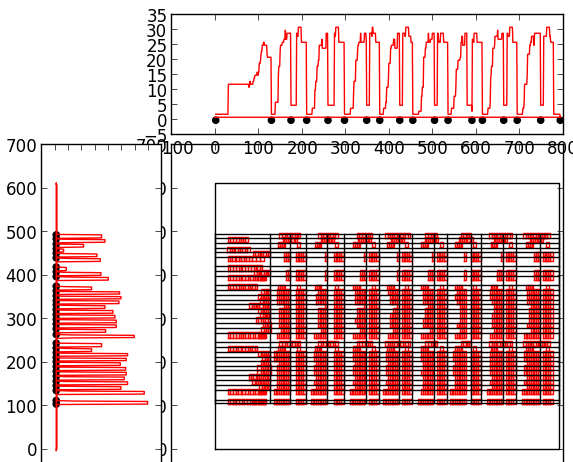
\includegraphics[scale=0.38]{ch3-images/projplot}}
							\caption{Inférence des frontières de la table de la figure \ref{fig:IFA-PDF}.}
							\label{fig:projplot}
						\end{wrapfigure}
	Pour trouver ces lignes verticales et ces colonnes, nous projetons les boites bleues (textuelles)sur l'axe horizontal (pour retrouver les colonnes\footnote{Nom du pays exportateur}) et sur l'axe vertical (pour retrouver les lignes\footnote{Données des enregistrements-ventes effectués par un pays importateur }). La projection consiste en l'énumération du nombre de boites bleues le long d'une ligne horizontale ou verticale. Nous concluons ainsi que les frontières entre les colonnes et les lignes sont marquées par les creux des valeurs des projections dans le graphe de projection; alors que les colonnes et les lignes en elles-même représentent les pics de la courbe. La figure \ref{fig:projplot} montre le résultat du traitement de la page de la figure \ref{fig:IFA-PDF}.\\Les graphes en haut et à gauche représentent le décompte des projections alors que les points noirs représentent les endroits où nous allons placer les frontières des lignes et des colonnes.
	\subsubsection{Conception du flux de données du processus de consolidation} \label{struct}
	La nature des transformations à faire subir les sources de données en vue de leur consolidation, nous amène à concevoir une solution technique en 2 phases:
	\begin{enumerate}
	\item \textbf{Une phase de structuration des données\footnote{cf. Annexe B1 pour le code-source}:}
	\begin{itemize}
	\item Nous parcourons l'arborescence contenant les .pdf source.
	\item Nous séparons le fichier .pdf en pages individuelles.
	\item Nous analysons les premiers caractères de la page en vue de labelliser chaque page selon si elle contient un produit, quel trimestre traite-elle, quelle normes les chiffres rapportés suivent-ils (cf. figure \ref{fig:IFA-TXT}).
	\item Nous faisons appel à notre outil de détection des tables discuté plus haut pour transformer chaque page-produit en une matrice de données.
	\item Nous compilons les matrices données d'un même produit en un seul fichier "data.csv" que nous confions au gestionnaire de fichier à placer dans une arborescence codifiant les données fonctionnelles de chaque fichier\footnote{cf. Annexe B3 pour plus de détails}.
	\end{itemize}
	\item \textbf{Une phase d'unification des modèles de données\footnote{cf. Annexe B2 pour le code-source}:}
	\begin{itemize}
	\item Nous parcourons l'arborescence générée par la phase précédente pour lire l'ensemble des "data.csv".
	\item Nous interrogeons le systèmes de fichier lors de la récupération de "data.csv" quant aux données fonctionnelles de celui-ci.
	\item Nous procédons si besoin aux opérations de décumulation et conversion.
	\item Les champs sont remplis conformément au modèle datamart OCP-CM (cf. figure \ref{fig:DMOCP}) et les données sont ainsi unifiées après audit de leur qualité.
	\end{itemize}
	\end{enumerate}
	Ces étapes sont résumées par le diagramme de flux de données de la figure \ref{fig:DF}.
		\begin{figure}[h]
		    		\centering
		    		\fbox{\includegraphics[scale=0.575]{ch3-images/dataflow}}
		    		\caption{Flux de données du processus de consolidation.}
		    		\label{fig:DF}
		\end{figure}
	\subsection{Audit et description des données locales consolidées}
	\subsubsection{Audit des données de consolidation}
	Lors de nos tests de la solution que nous avons mis au point lors de la section \ref{parser}, nous obtenions un taux de réussite de reconnaissance et extraction des tableau de 100\%. Cependant et de par la nature critique des données que nous traitons, nous avons procédé à tes tests rigoureux de deux natures différentes.
	\paragraph{Audit assisté par ordinateur:\\}
	Notre processus de consolidation a généré en moyenne près de 40800 enregistrements-vente par année. Après une consolidation des années 2014, 2015 et début 2016, le total s'élève à 94240 nouveaux enregistrements-vente dont nous nous devons d'assurer la justesse. Une vérification humaine un par un de chacun de ces enregistrements-vente est une tâche pharamineuse que nous taclons en premier lieu en nous assistons du langage \textbf{R\footnote{\textbf{R} est un langage de programmation, de traitement des données et d'analyse statistique mettant en œuvre le langage de programmation \textbf{S}, avec la sémantique dérivée du langage \textbf{Scheme}}}.
\paragraph{}
		La figure \ref{fig:size} ci-dessous, valide bien le nombre d'enregistrements-vente auxquels on s'attend, soit 94240 lignes. De plus, nous remarquons un premier soucis : Les cases de volumes nuls au sein de la colonne "kT" de la Trade Matrix ont été interprétés par le caractère "-". Ce qui empêche la colonne d'être traitée en tant que vecteur numérique. Nous remédions à ce problème en remplaçant ce caractère par le numérique "0", comme procédé dans la figure \ref{fig:nas} ci -après.
		\newline
			\begin{figure}[H]
			\begin{subfigure}{.5\textwidth}
				\centering
				\fbox{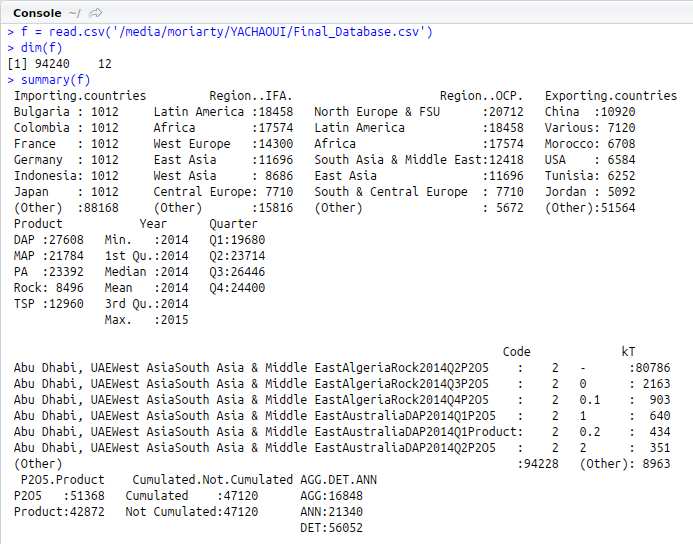
\includegraphics[height=215pt]{ch3-images/1}}
				\caption{Vérification de la dimension\\des données consolidées}
				\label{fig:size}
			\end{subfigure}
			\begin{subfigure}{.5\textwidth}
					\centering
					\fbox{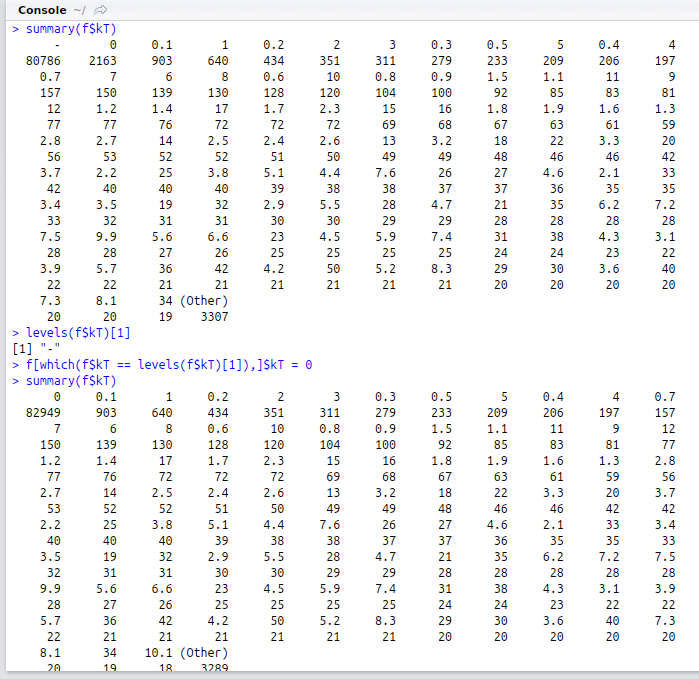
\includegraphics[height=215pt]{ch3-images/2}}
					\caption{Traitement des cases vides\\des données consolidées}
					\label{fig:nas}
			\end{subfigure}
			\caption{Audit : Dimensions et données manquantes.}
				\end{figure}
				
	\paragraph{}
	Dans les figures \ref{fig:dubai} et \ref{fig:taiwan}, Nous observons deux interprétation différentes de \textbf{Dubai} en ("\textit{Dubai, UAE}","\textit{Dubai/ UAE}") et de \textbf{Taiwan} en ("\textit{Taiwan, China}","\textit{Taiwan/ China}"). Ces discrépances seraient analysées en tant que 4 pays différents alors qu'en réalité, ceux-ci ne sont que deux.\\Nous procédons à la correction de ces deux ambiguïtés dans les figures \ref{fig:corrDubai} et \ref{fig:corrTaiwan} respectivement.
	\par
	Un malfonctionnement similaire est à noter pour les drapeaux de la colonne \textit{P2O5.Product}\footnote{Drapeau indiquant si le poids indiqué à la colonne \textit{kT}est net en P2O5 ou en poids brut.} où des caractères "\textbf{espace}" se sont introduits en début de chaîne pour proposer ici aussi 4 niveaux qualitatifs  au lieu de 2 uniquement.\\Nous diagnostiquons ce soucis et le corrigeons dans la figure \ref{fig:corr}
	\begin{figure}[H]
	\begin{subfigure}{.5\textwidth}
			\centering
			\fbox{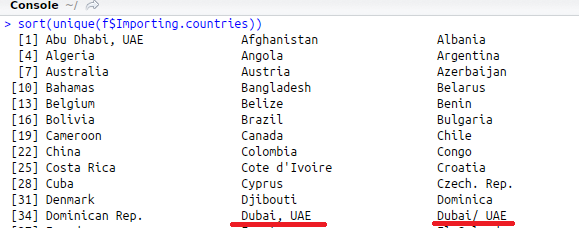
\includegraphics[height=90pt]{ch3-images/4}}
			\caption{Ambiguïté Dubai, UAE}
			\label{fig:dubai}
	\end{subfigure}
	\begin{subfigure}{.5\textwidth}
		\centering
		\fbox{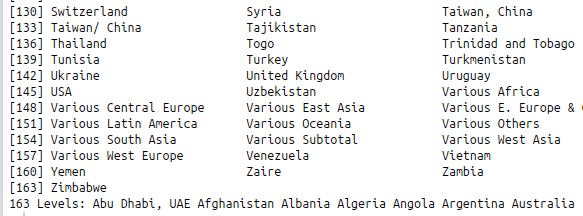
\includegraphics[height=90pt]{ch3-images/5}}
		\caption{Ambiguïté Taiwan, China}
		\label{fig:taiwan}
	\end{subfigure}
	\begin{subfigure}{\linewidth}
			\centering
			\fbox{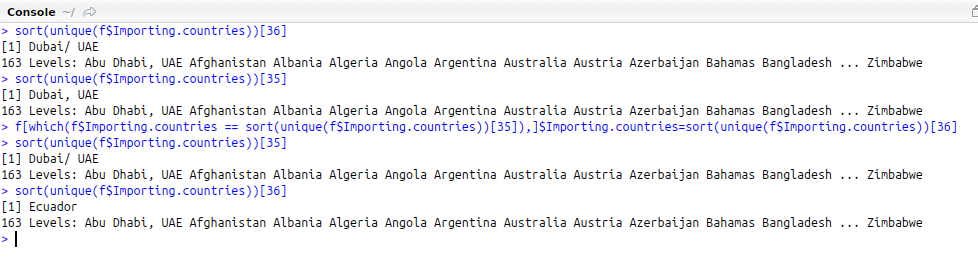
\includegraphics[width=\linewidth]{ch3-images/6}}
			\caption{Correction Dubai, UAE}
			\label{fig:corrDubai}
	\end{subfigure}
	\begin{subfigure}{\linewidth}
			\centering
			\fbox{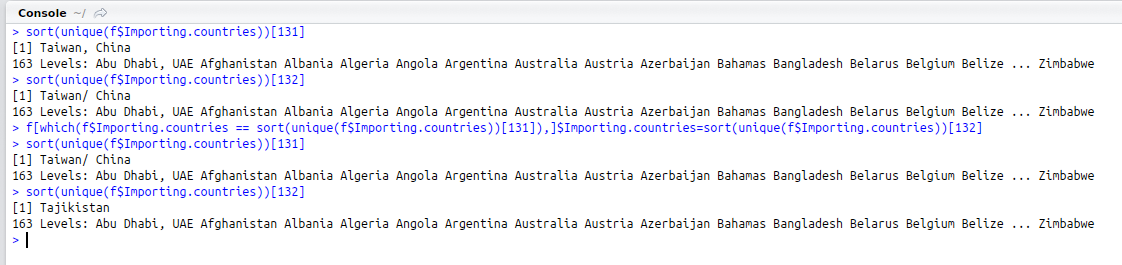
\includegraphics[width=\linewidth]{ch3-images/7}}
			\caption{Correction Taiwan, China}
			\label{fig:corrTaiwan}
	\end{subfigure}
		\begin{subfigure}{\linewidth}
			\centering
			\fbox{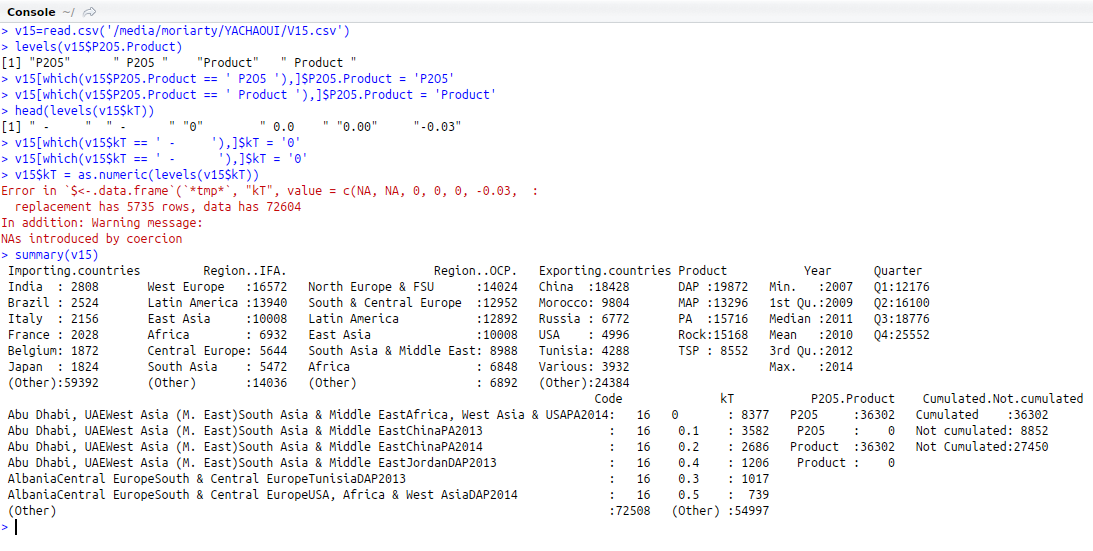
\includegraphics[width=\linewidth]{ch3-images/10}}
			\caption{Correction des drapeaux de la colonne \textit{P2O5.Product}}
			\label{fig:corr}
		\end{subfigure}
			\caption{Audit: Interprétation des chaînes de caractères.}
			\end{figure}
		\begin{figure}[H]
%		\begin{subfigure}{\linewidth}
		\centering
		\fbox{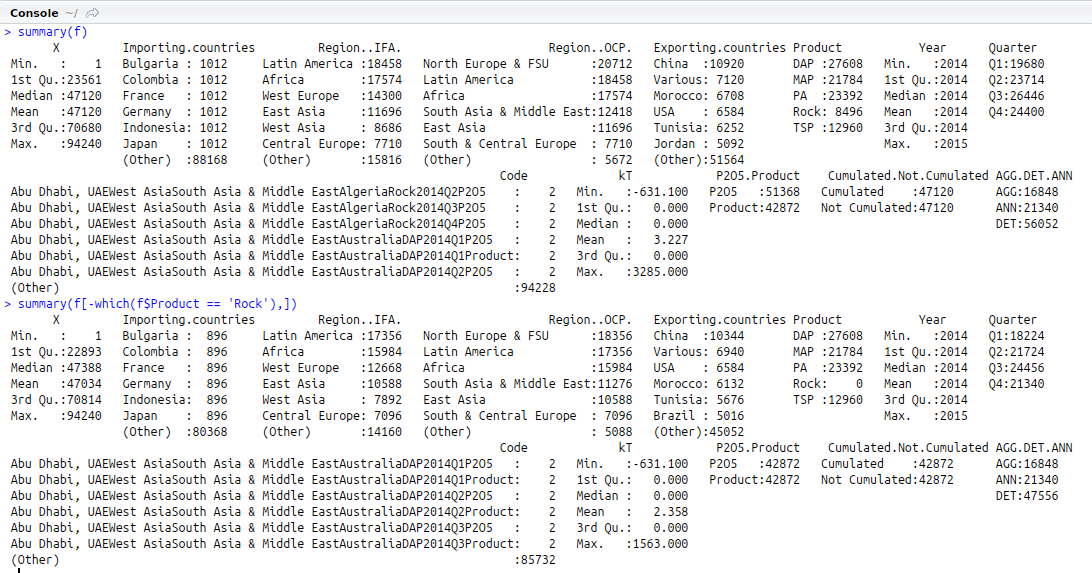
\includegraphics[width=0.925\linewidth]{ch3-images/8}}
		\caption{Audit: Conversion des unités de mesures.}
		\label{fig:diffprod}
		\end{figure}
		La figure \ref{fig:diffprod} ci-dessous, relève un écart de 51368-42872 = 8496 enregistrements-vente de plus possédant le drapeau \textit{Product} et pas le drapeau \textit{P2O5}. Ce chiffre nous interpelle puisque celui-ci est justement celui d'enregistrements-vente \textbf{Product == "Rock"}. Dans la figure \ref{fig:corrprod}, nous investiguons cette fausse coïncidence en nous nous intéressons uniquement aux enregistrements-vente  \textbf{Product $\neq$ "Rock"} où il s'avère que cet écart n'est plus. Ceci nous amène à ajuster notre code de conversion présenté dans la phase d'unification à la section \ref{struct}.
		\begin{figure}[H]
		\centering
		\fbox{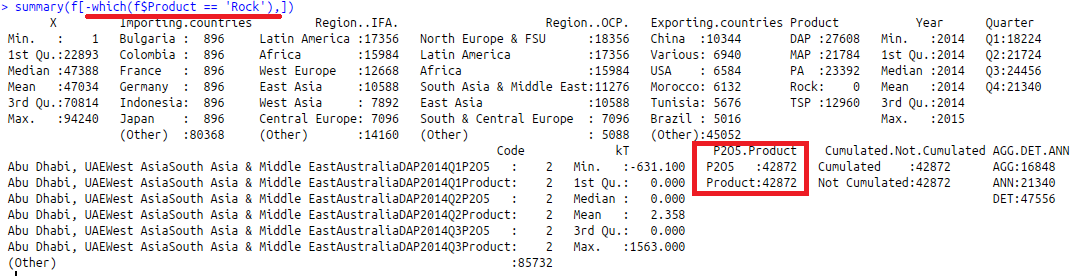
\includegraphics[width=\linewidth]{ch3-images/8bis}}
		\caption{Audit: Correction des unités de mesures.}
		\label{fig:corrprod}
		\end{figure}
	\paragraph{Audit manuel d'échantillons aléatoires:\\}
	Une vérification supplémentaire a été entreprise par nos soins, en choisissant aléatoirement:
	\begin{itemize}
	\item Une année d'exercice,
	\item Un semestre d'exercice,
	\item Un produit phosphaté,
	\item Un pays importateur.
	\end{itemize}
	Nous listons l'ensemble des imports de celui-ci que nous avons consolidé qu'on compare par la suite visuellement aux fichier .pdf de départ en termes de:
	\begin{itemize}
	\item Poids rapporté,
	\item Drapeaux et normes de l'enregistrement-vente,
	\item Adéquation des chaînes de synthèse de la colonne \textit{Code}.
	\end{itemize}
	Pour un échantillon de 20 tirages, nous n'avons observé aucun écart.
	\subsubsection{Description des données de consolidation}
	Nous procédons dans la partie suivante à la visualisation exploratoire de nos données consolidées. En statistiques, l'analyse exploratoire des données (AED) est une approche de l'analyse des ensembles de données pour résumer leurs principales caractéristiques, souvent avec des méthodes visuelles. Un modèle statistique peut être utilisé ou non, mais surtout l'AED interrogent les données sur ce qu'elles peuvent nous dire au-delà de la modélisation formelle ou des tâches de vérification d'hypothèses. Le script en langage \textbf{R} de l'AED à suivre peut être retrouvé dans le dossier \textit{Source} du dépôt \textbf{GitHub} de notre mémoire de projet de fin d'études\cite{this}.
	\paragraph{Description des quantités exportées\\}
	La figure \ref{fig:BAM} ci-dessous est la représentation graphique des distributions des échanges mondiaux des produits. Nous nous intéressons ainsi à la colonne \textit{kT} du datamart de la figure \ref{fig:DMOCP}. Nous procédons en un premier lieu à la transformation logarithmique de cette colonne en vue d'atténuer les écarts entre les valeurs les plus extrêmes et produire des diagramme visuellement plus plaisants offrant plus de flexibilité à l'interprétation. Les diagramme de la figure \ref{fig:BAM} sont communément appelés des \textit{Boites à Moustaches} et résument l'information de dispersion des valeurs tracées par une boite (en rouge) délimitée par l'écart interquartile $Q_3 - Q_1$ représentant les enregistrements séparant les 25\% des valeurs les plus extrêmes et dont la ligne centrale représente la moyenne de l'échantillon. Les moustaches de la boite permettent de se prononcer quant aux valeurs aberrantes : sont coloriées en Orange, les valeurs dépassant les limites des moustaches dont la longueur est (1.5 x $Q_3 - Q_1$).
			\begin{figure}[H]
			\centering
			\fbox{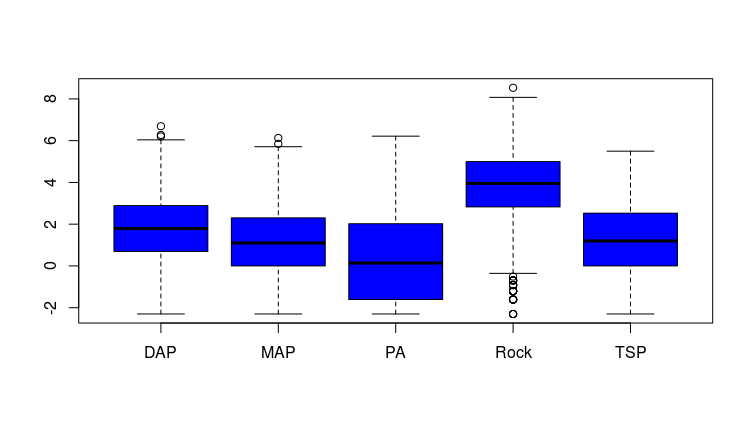
\includegraphics[width=\linewidth]{ch3-images/A}}
			\caption{Boites à moustaches des quantités logarithmiques exportées par produit phosphatés. Gauche : Quantités mondiales. Droite : Exports Marocains.}
			\label{fig:BAM}
			\end{figure}
			\newpage
			De par les lignes centrales des boites, il s'avère que le Maroc exporte nettement plus que la moyenne mondiale en acide phosphorique (PA), en roche (Rock); dépasse sensiblement les moyennes DAP et MAP, et sous-performe dans les exports des TSP. Nous prêterons plus d'attention aux histogrammes de la figure \ref{fig:HistProd} ci-dessous en les contextualisant au sein des rôles des exportateurs majeurs de produits phosphatés. Nous nous suffirons ici de relever que ces histogrammes confirment bien la rareté des valeurs aberrantes ressortant après notre transformation logarithmique : 
			\begin{figure}[H]

						\begin{subfigure}{.5\textwidth}
								\centering
								\fbox{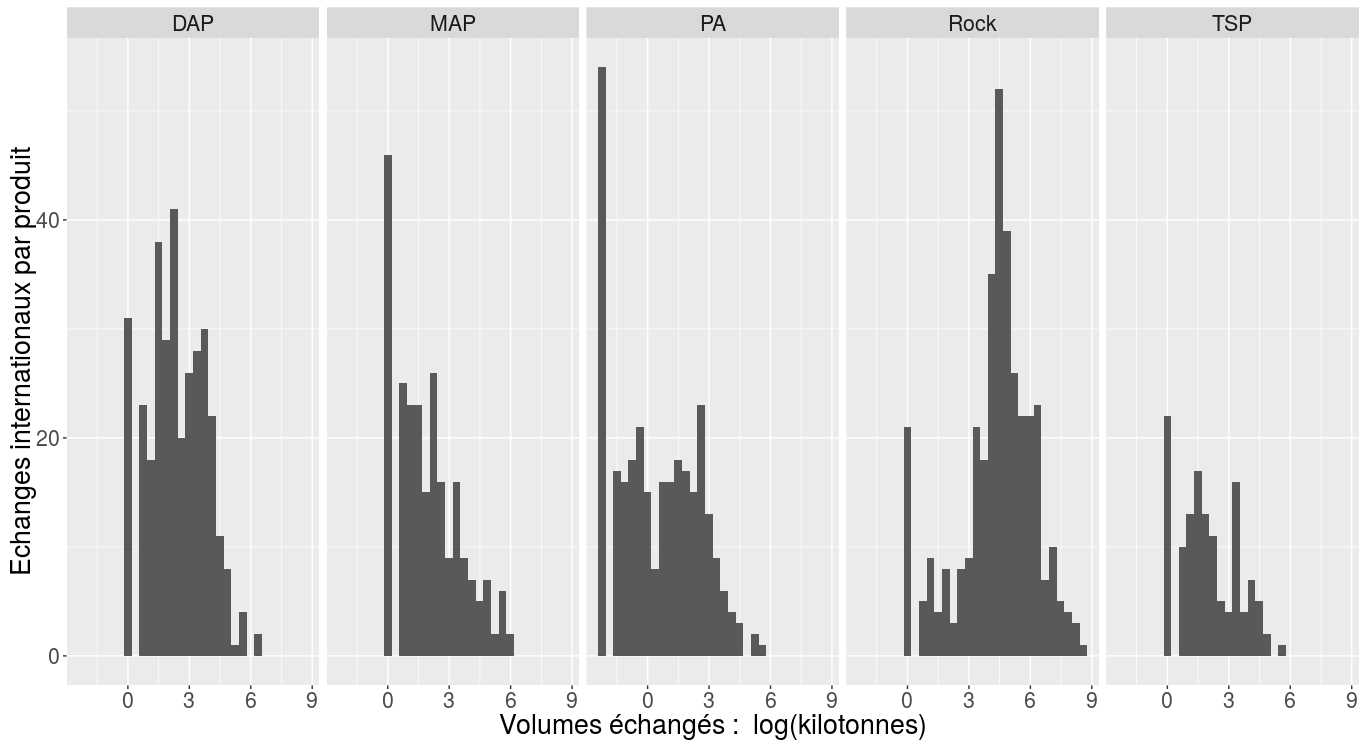
\includegraphics[width=\textwidth]{ch3-images/G}}
								\caption{Histogramme des quantités logarithmiques mondiales exportées par produit.}
								\label{fig:}
						\end{subfigure}
						\begin{subfigure}{.5\textwidth}
												\centering
												\fbox{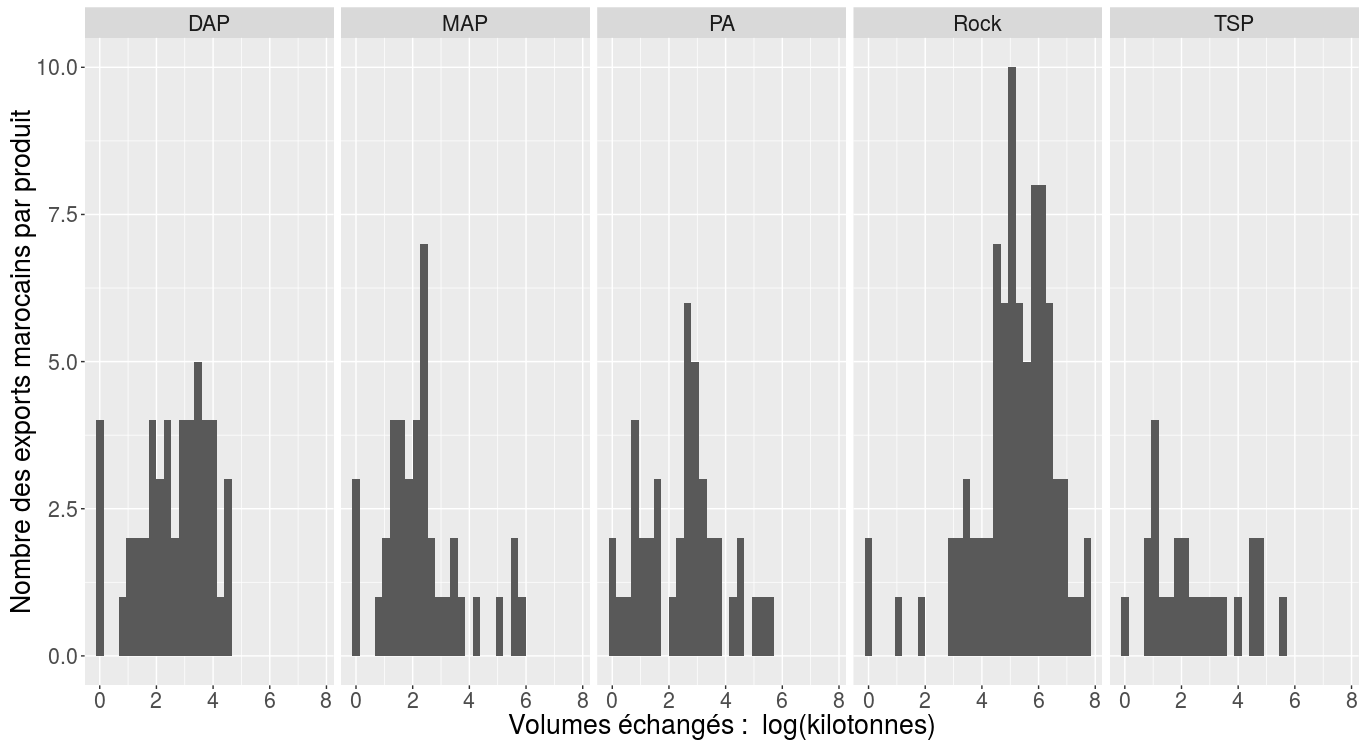
\includegraphics[width=\textwidth]{ch3-images/H}}
												\caption{Histogramme des exports logarithmiques\\Marocains par produit.}
												\label{fig:}
						\end{subfigure}
						\caption{Histogramme des quantités logarithmiques exportées par produit.}
						\label{fig:HistProd}
					\end{figure}
		\paragraph{Description des exportateurs majeurs\\}
		Nous nous proposons dans la section suivante d'étudier de plus près la position du Maroc au sein des exportateurs majeurs de produits phosphatés. Nous empilons les histogrammes des produits de la figure \ref{fig:HistProd} en coloriant les barres selon le produit concerné (figure \ref{fig:colprod}) et les exportateurs les ayant émis (figure \ref{fig:colexp}). La figure \ref{fig:DistProdExp} permet les observations suivantes:
		\begin{enumerate}
		\item Observations relatives au type de produits exportés:
			\begin{itemize}
			\item Les volumes d'acide phosphorique sont échangés par lot de petites quantités. Ceci s'explique d'une part par la spécificité des besoins en acide qui ne couvrent qu'un ensemble réduit d'industries; et d'une autre part par les précautions contraignantes à observer durant le fret de l'acide. La figure \ref{fig:densprod} montre bien un pic au niveau des plus faibles valeurs des quantités exportées.
			\item Les fertilisants DAP, MAP et TSP sont similairement centrés. L’explication est à corréler avec la généricité des applications agricoles de ceux-ci ainsi que le volume transportable par les cargo maritimes de type \textit{Panamax}\cite{ocp-fil}.
			\item Les volumes des lot de roche de phosphate s'articule largement au-dessus du reste des produits et est possiblement imputable au format de transport de la roche - en vrac - qui ne nécessite par de dispositions particulières lors du transport maritime ainsi que la nécessité pour les pays importateurs de disposer d'usine de traitement de la roche, exemple d'industrie qui acquiert sa matière première en contrat annuels\cite{ocp-fil}.
			\end{itemize}
		\newpage
		\item Observations relatives aux positionnement des exportateurs majeurs:
			\begin{itemize}
		\item La Chine s'est forgée un marché de lots d'export de faibles quantités mais plus grand en fréquence. Ce positionnement est représenté par la courbe chinoise sur la figure \ref{fig:colexp} et éclairci par la figure \ref{fig:destReg} qui présente une Chine dominant le marché asiatique caractérisé par un nombre élevé de pays-clients différents.
		\item Dans les livraisons à grand volume, le Maroc est incontestablement favori, surclassant ainsi la Russie et les USA dans la figure \ref{fig:colexp}
			\end{itemize} 
		\end{enumerate} 
		\begin{figure}[H]
		\begin{subfigure}{.5\textwidth}
				\centering
				\fbox{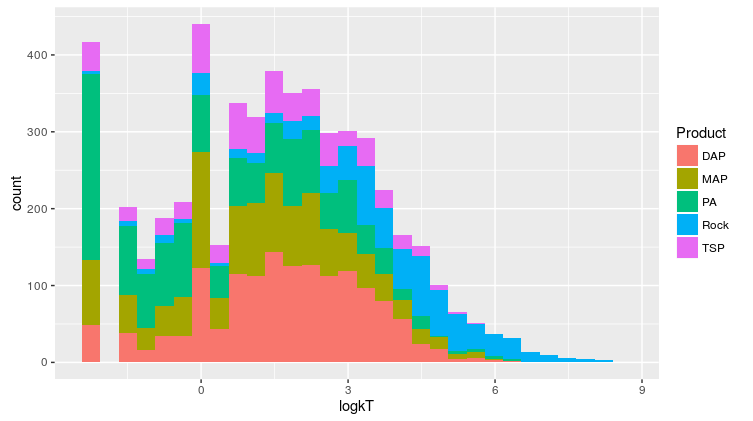
\includegraphics[width=\textwidth]{ch3-images/B}}
				\caption{Histogramme des quantités logarithmiques mondiales exportées par produit.}
				\label{fig:colprod}
		\end{subfigure}
		\begin{subfigure}{.5\textwidth}
				\centering
				\fbox{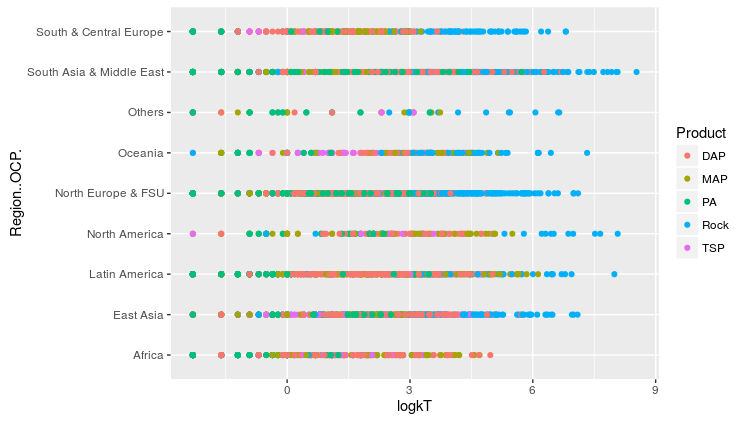
\includegraphics[width=\textwidth]{ch3-images/D}}
				\caption{Histogramme des quantités logarithmiques mondiales exportées par exportateur majeur.}
				\label{fig:colexp}
		\end{subfigure}
				\begin{subfigure}{.5\textwidth}
						\centering
						\fbox{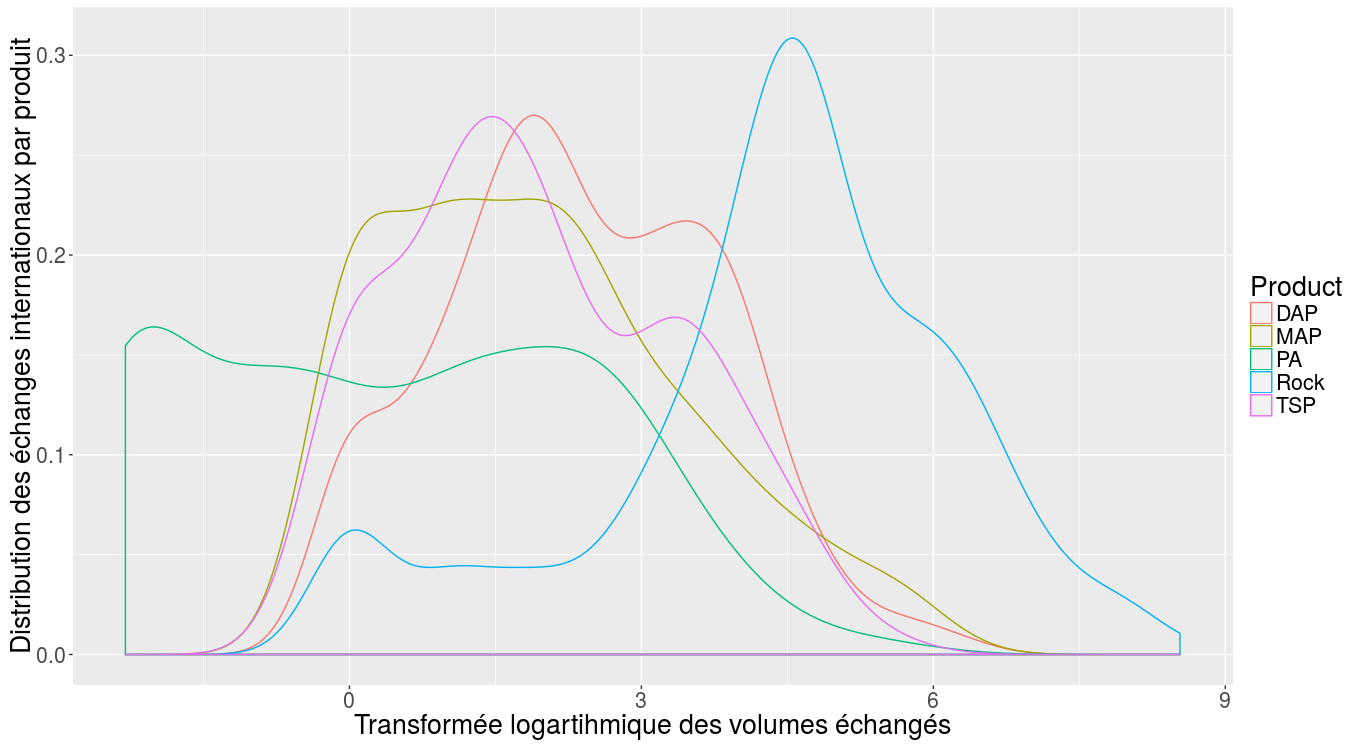
\includegraphics[width=\textwidth]{ch3-images/C}}
						\caption{Densités des quantités logarithmiques\\mondiales exportées par produit.}
						\label{fig:densprod}
				\end{subfigure}
				\begin{subfigure}{.5\textwidth}
						\centering
						\fbox{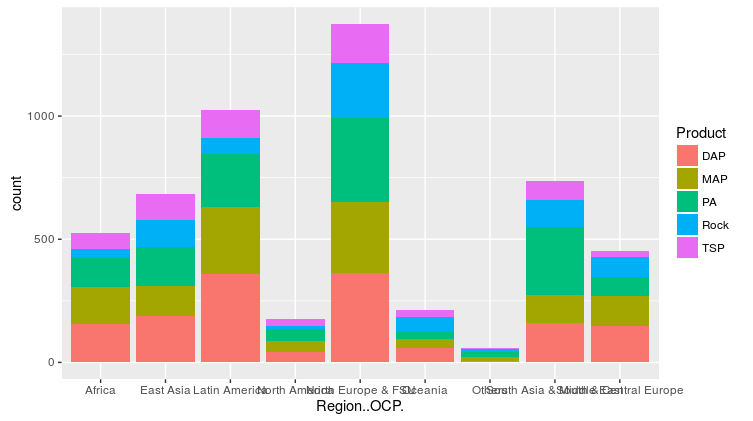
\includegraphics[width=\textwidth]{ch3-images/E}}
						\caption{Densités des quantités logarithmiques\\mondiales exportées par exportateur majeur.}
						\label{fig:densexp}
				\end{subfigure}
						\caption{Distributions des quantités logarithmiques mondiales exportées par produit et par exportateur majeur.}
						\label{fig:DistProdExp}
		\end{figure}
		\paragraph{Description des régions importatrices\\}
		Nous
				\begin{figure}[H]
				\centering
				\fbox{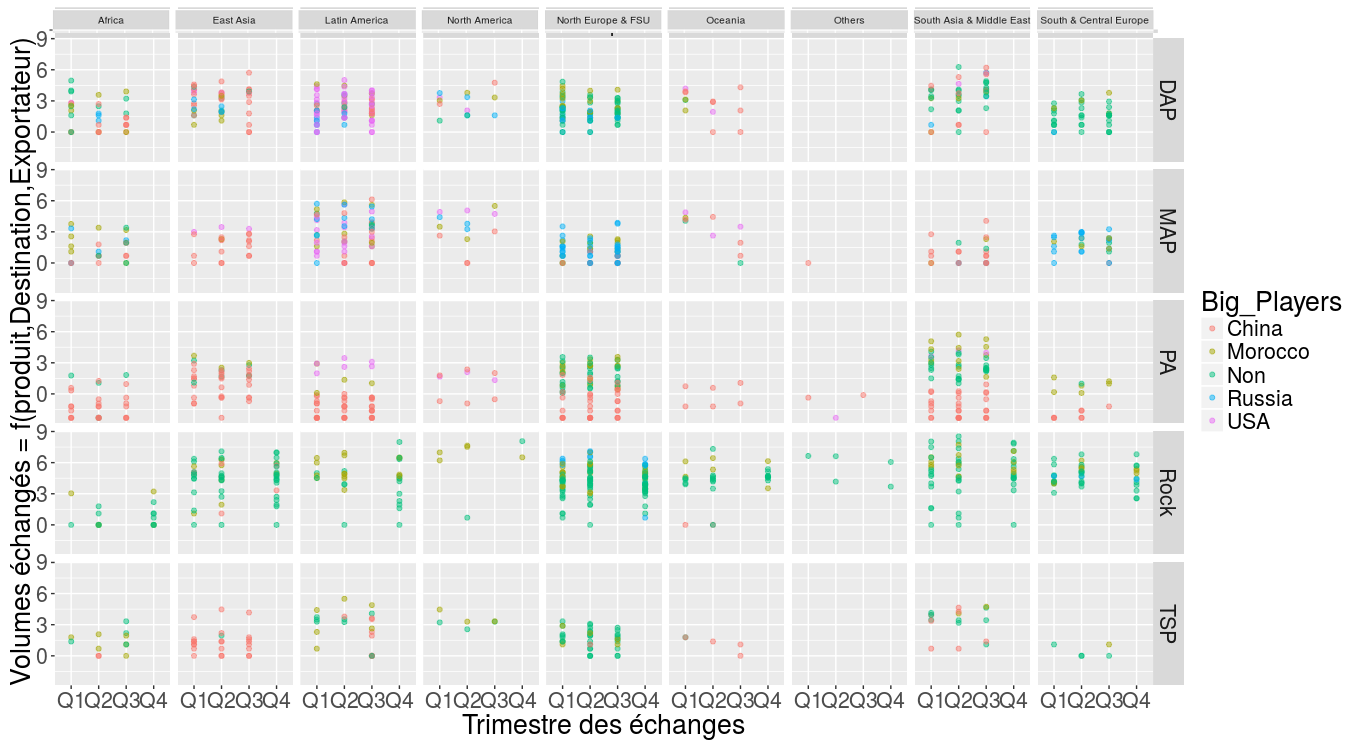
\includegraphics[width=\linewidth]{ch3-images/J}}
				\caption{}
				\label{fig:destReg}
				\end{figure}	
				\begin{figure}[H]
				\centering
				\fbox{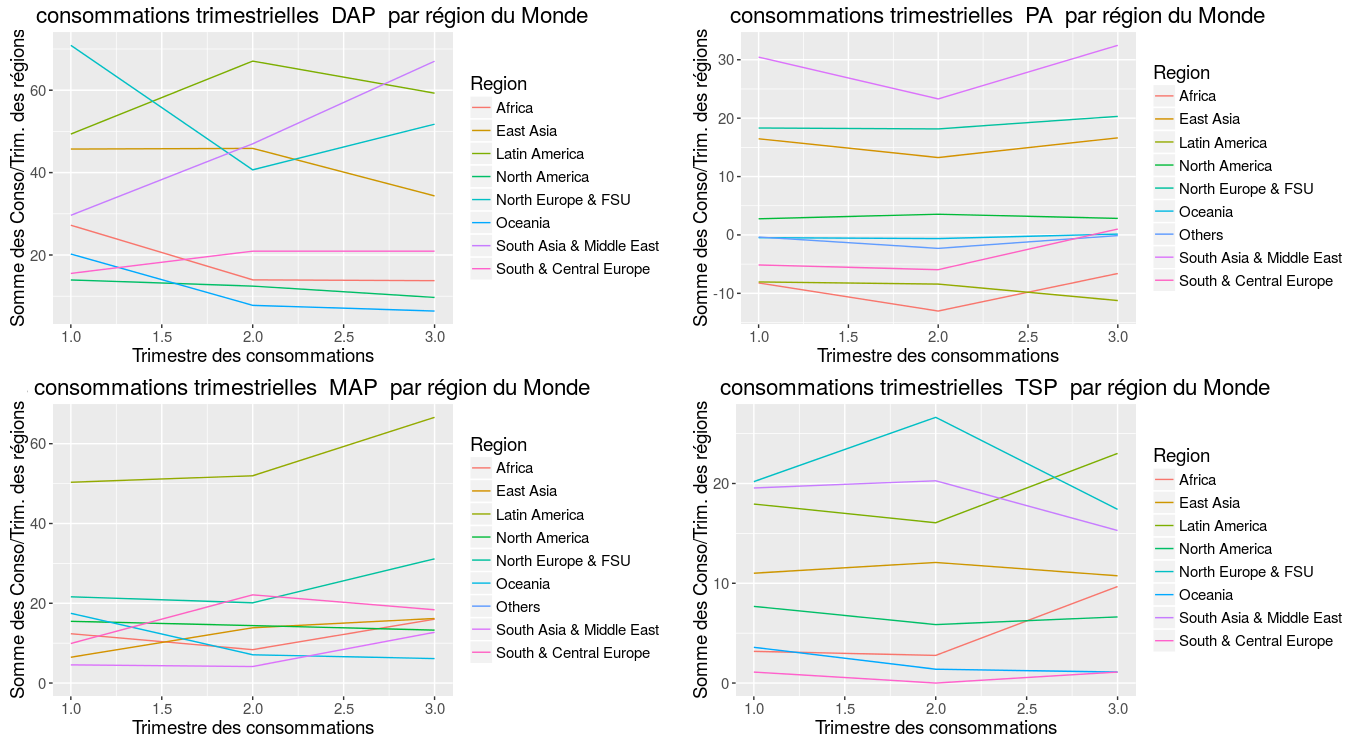
\includegraphics[width=\linewidth]{ch3-images/K}}
				\caption{}
				\label{}
				\end{figure}

	\section{Collecte et préparation des données externes}
	L'étendue des données disponibles au sein du système d'information de l'OCP ne pouvant donner qu'une vue réduite de la situation du marché et ne peuvent de par leur définition révéler les structures socio-économiques,  et de politiques agraires sous-jacentes aux demandes en produits phosphatés, nous nous attellerons à la tâche d'enrichir cette base de données historiques par des données quantitatives concernant les pays du monde.
	\par
	Nous décrivons dans ce qui suit ce processus. 
	\subsection{Collecte des données externes}
	\subsubsection{Énumération et définitions des variables souhaitées }\label{exoList}
			Guidés par nos lectures bibliographiques résumées dans les sections \ref{read1} et \ref{read2}, nous nous fixons l'objectif de récolter les indicateurs de politiques agraires et socioéconomiques suivants:
	\begin{itemize}
		\item \textbf{ Access to electricity, rural (\% of rural population):} Fraction de paysans ayant accès à l'électricité.
		\item \textbf{ Access to non-solid fuel, rural (\% of rural population):} Fraction de paysans ayant accès aux fuels non solides.
		\item \textbf{ Account at a financial institution (\% age 15+):} Fraction de personnes âgées de +15 ans ayant un compte chez une institution bancaire.
		\item \textbf{ Net enrollment rate, primary (\% of primary school age children):} Fraction d'enfants scolarisés.
		\item \textbf{ Net national income per capita (constant 2005 US\$):} PIB\footnote{Produit intérieur brut, un des agrégats majeurs des comptes nationaux, il vise à quantifier — pour un pays et une année donnés — la valeur totale de la « production de richesse » effectuée par les agents économiques résidant à l’intérieur de ce territoire (ménages, entreprises, administrations publiques).} par habitant, inflation ajustée au dollar US fin 2005.\nomenclature{\textbf{PIB : }}{Produit intérieur brut}
		\item \textbf{ Literacy rate, adult total (\% of people ages 15 and above):} Fraction de personnes alphabétisées âgées de +15ans.
		\item \textbf{ Agricultural irrigated land (\% of total agricultural land):} Fraction de terres irriguées parmi les terres exploitées pour l'agriculture.
		\item \textbf{ Agricultural land (\% of land area):} Fraction des terres agricoles de la surface totale du pays.
		\item \textbf{ Agricultural tractors per 100 sq. km of arable land:} Nombre de tracteurs par 100 km² de terres arables.
		\item \textbf{ Agriculture, value added (\% of GDP):} Fraction de la valeur ajoutée agricole du PIB.
		\item \textbf{ Agriculture value added per worker (constant 2005 US\$):} Valeur ajoutée agricole par ouvrier agricol, inflation ajustée au dollar US fin 2005.
		\item \textbf{ All education staff compensation, total (\% of total expenditure in public institutions):} Fraction des dépenses en éducation des dépenses en institutions publiques.
		\item \textbf{ Annual freshwater withdrawals, agriculture (\% of total freshwater withdrawal):} Fraction du volume d'eau utilsée à des fins agricoles de la totalité de l'eau consommée.
		\item \textbf{ Arable land (\% of land area):} Fraction de terres arables de la surface totale du pays.
		\item \textbf{ Arable land (hectares per person):} Nombre d'hectares de terres arables par personne.
		\item \textbf{ Birth rate, crude (per 1,000 people):} Nombre de naissances par 1000 personnes.
		\item \textbf{ Cereal yield (kg per hectare):} Rendement des céréales en kilogramme par hectare.
		\item \textbf{ Commercial bank branches (per 100,000 adults):} Nombre d'agences bancaires par 100,000 adultes.
		\item \textbf{ Consumer price index (2010 = 100):} L'indice des prix à la consommation (IPC) mesure l'évolution du niveau moyen des prix des biens et services consommés par les ménages, pondérés par leur part dans la consommation moyenne des ménages. Harmonisé pour permettre une comparaison entre les pays à fin 2010.
		\item \textbf{ Cost to export (US\$ per container):} Coût en Dollars US de l'export d'un conteneur de marchandises.
		\item \textbf{ Cost to import (US\$ per container):} Coût en Dollars US de l'import d'un conteneur de marchandises.
		\item \textbf{ Crop production index (2004-2006 = 100):} 
		L'indice de production des cultures montre la production agricole pour chaque année par rapport à la période de base de 2004 à 2006. Cet indice porte sur l'ensemble des cultures à l'exception des cultures fourragères. Les regroupements par région et par revenu des indices de production de la FAO\nomenclature{\textbf{FAO : }}{Food and Agriculture Organization of the United Nations} sont calculés à partir des valeurs sous-jacentes en dollars US et normalisés par rapport à la période de référence de 2004 à 2006.
		\item \textbf{ Droughts, floods, extreme temperatures (\% of population, average 1990-2009):} Pourcentage moyen annuel entre 1990 et 2009 de la population affectée par les catastrophes naturelles classifiées comme sécheresses, inondations et évènements climatiques extrêmes.
		\item \textbf{ Employment in agriculture (\% of total employment):} Fraction des ouvriers agricoles de l'ensemble des employés.
		\item \textbf{ Food production index (2004-2006 = 100):} L'indice de production alimentaire porte sur les cultures vivrières qui sont considérées comme comestibles et qui contiennent des nutriments et normalisées par rapport à la période de référence de 2004 à 2006.
		\item \textbf{ GDP per capita (constant 2005 US\$):} PIB par habitant. Inflation ajustée à fin 2005.
		\item \textbf{ Household final consumption expenditure (constant 2005 US\$):}  La consommation privée désigne la valeur marchande de tous les biens et services, y compris les produits durables achetés par les ménages.
		\item \textbf{ Lending interest rate (\%):} Le taux d'intérêt perçu par les banques sur les prêts accordés aux clients.	
		\item \textbf{ Life expectancy at birth, total (years):} L'espérance de vie à la naissance indique le nombre d'années qu'un nouveau-né devrait vivre si les règles générales de mortalité au moment de sa naissance devaient rester les mêmes tout au long de sa vie.
		\item \textbf{ Livestock production index (2004-2006 = 100):} L'indice de production animale comprend la production de viande et de lait de toutes sources, les produits laitiers tels que le fromage, les œufs, le miel, la soie brute, la laine ainsi que les peaux et les cuirs.
		\item \textbf{ Logistics performance index:} La note globale de l'indice de performance de la logistique reflète les perceptions relatives à la logistique d'un pays basées sur l'efficacité des processus de dédouanement, la qualité des infrastructures commerciales et des infrastructures de transports connexes, la facilité de l'organisation des expéditions à des prix concurrentiels, la qualité des services d'infrastructure, la capacité de suivi et de traçabilité des consignations et la fréquence avec laquelle les expéditions arrivent au destinataire dans les délais prévus. L'indice varie continuellement de 1 à 5 et la note la plus élevée représente la meilleure performance.
		\item \textbf{ Low-birthweight babies (\% of births):} Fraction des nouveau-nés pesant moins de 2 500 grammes des naissances totales.
		\item \textbf{ Net migration:} Nombre d'immigrants total moins le nombre d'émigrants annuel, comprenant à la fois les citoyens et les non citoyens.
		\item \textbf{ Permanent cropland (\% of land area):} Fraction des terres occupées par des cultures pour de longues périodes et qui doivent être replantées après chaque récolte de la surface totale du pays.
		\item \textbf{ Population density (people per sq. km of land area):} Densité des habitants en personne par km².
		\item \textbf{ Population growth (annual \%):} Croissance relative annuelle de la population.
		\item \textbf{ Rural population (\% of total population):} Fraction rurale de la population.
		\item \textbf{ Rural poverty gap at national poverty lines (\%):} L'écart de pauvreté par rapport au seuil national de la pauvreté en milieu rural est le manque à gagner pour remonter au-dessus du seuil de la pauvreté (en considérant que les non pauvres ont un manque à gagner de zéro) exprimé en pourcentage du seuil national de la pauvreté en milieu urbain.Cette mesure témoigne à la fois de l'ampleur de la pauvreté et de sa fréquence.
		\item \textbf{ Unemployment, total (\% of total labor force):} Fraction de la population active qui est sans emploi mais qui est disponible pour et à la recherche d'un emploi.
		\end{itemize}
	\subsubsection{Énumération des sources WEB des variables souhaitées}
	\par
	\begin{Huge}{ Liste des cibles  web et bases de données publiques}
		\end{Huge}

	\subsection{Préparation des données externes}
	Cette section s’intéresse à l'application des forêts de décisions aléatoires à des fins de sélection de variables. Le but ici est double : d'abord introduire le comportement de l'indexation de l'importance des variables en utilisant les forêts aléatoires et l'utiliser pour proposer un algorithme à deux phases pour la sélection de variables à la base de leur importance.\par
	La stratégie générale se résume en un classement des variables exogènes\footnote{à savoir les variables externes énumérées dans la section \ref{exoList}}. en utilisant le score d'importance de ces variables introduit par les forêts aléatoires puis une sélection ascendante itérative des variables.
	\subsubsection{Introduction à la selection de variables via forêts de décision aléatoires}
	Les FA\nomenclature{\textbf{FA : }}{Forêts aléatoires} est un algorithme populaire et très efficient basé appartenant aux méthodes d'agrégation pour les problèmes de régression et de classification, introduit par Breiman\cite{BREI01}, et apparaît dans les application de 'Machine Learning'\footnote{L'apprentissage automatique ou apprentissage statistique (machine learning en anglais), champ d'étude de l'intelligence artificielle, concerne la conception, l'analyse, le développement et l'implémentation de méthodes permettant à une machine (au sens large) d'évoluer par un processus systématique, et ainsi de remplir des tâches difficiles ou impossibles à remplir par des moyens algorithmiques plus classiques.} à la fin du dernier millénaire\cite{DITRI99}. Les FA deviennent de plus en plus populaires et semblent être très robustes dans beaucoup d'applications bien qu'ils ne soient pas clairement théorisés mathématiquement\cite{BIA08}. Une introduction sommaire des FA est donnée en annexe A1.
	\par

	Le principe des FA est de combiner plusieurs arbres ($ê_i$) de décision CART\cite{BREI84} en utilisant plusieurs échantillons bootstrap de l'ensemble d'apprentissage \textbf{$L_n$} et de choisir aléatoirement à chaque nœud un sous-ensemble de \textit{k} variables exogènes $X_i$. 
	\par
	L'agrégation à laquelle procèdent les FA est d’autant plus performante que la corrélation entre les prédicteurs agrégés  (arbres CART\nomenclature{\textbf{CART : }}{Classification And Regression Trees}) est faible. Afin de diminuer cette corrélation, Breiman\cite{BREI01} propose de rajouter une couche d’aléa dans la construction des
	prédicteurs.  Nous attirons l'attention du lecteur vers l'annexe A2 pour une note sur CART et son utilisation au sein des FA. Sommairement, à chaque étape de CART, \textit{k} variables sont sélectionnées aléatoirement parmi les \textit{p} et la meilleure coupure est sélectionnée uniquement sur ces \textit{k} variables : \par
	\textbf{Algorithme Forêts aléatoires}
	\begin{itemize}
	\item[\textbf{Entrées:}]
	\item x, une nouvelle observation à prévoir.
	\item \textit{$L_n$}, l'échantillon.
	\item \textit{B}, le nombre d'arbres.
	\item \textit{k} $\in \mathbb{N}^* $, le nombre de variables candidates pour découper un nœud.
	\end{itemize}
	Pour i = 1,...,\textit{B}:
	\begin{itemize}
	\item Tirer un échantillon bootstrap dans \textit{$L_n$}.
	\item Construire un arbre CART sur cet échantillon bootstrap, chaque coupure est sélectionnée
	en minimisant la fonction de coût de CART sur un ensemble de \textit{k} variables choisies au
	hasard parmi les \textit{p}. On note $ê(.,\theta_i)$ l’arbre construit.
	\item[\textbf{Sortie:}]L’estimateur ${ê(x) =  \frac{1}{B} \sum_{i=1}^{B} ê_i(x,\theta_i)}$
	\end{itemize}	
	\subsubsection{Sélection des variables et élagage des données externes}
	Parmi les nombreuses sorties proposées par la fonction randomForest, deux se révèlent particulièrement intéressantes. \textbf{L'erreur Out-of-Bag} et \textbf{Le score FA d'importance des variables}. Nous définissons celles-ci rigoureusement dans l'annexe A3. Ces deux sorties nous permettent de proposer la procédure suivante à deux phases pour l'élimination itérative des variables les moins pertinentes:
	\paragraph{Phase 1. Élimination initiale et classement:}\begin{itemize}
	\item Nous modélisons par FA notre ensemble de données initial, comprenant la totalité des variables exogènes listées dans la section \ref{exoList}.
	\item Nous calculons les score FA d'importance des variables et nous éliminons les variables d'importance triviale.
	\item Nous classons les \textit{m} variables restantes par ordre descendant des score FA d'importance
	\end{itemize}
	\paragraph{Phase 2. Sélection des variables:}
	\begin{itemize}
	\item Nous construisons la collection itérative des modèles de FA employant les \textit{$\alpha$} premières variables selon leur classement de score d'Importance. Pour ${\alpha \in [1,\textit{m}]}$.
	\item Nous retenons les variables du modèle ayant réussi la plus faible erreur OOB.
	\end{itemize}
	